\chapter{Appendix}\label{chap:appendix}
\begin{table}[h]
    \begin{center}
    \caption{Assay source names and long names}
    \begin{tabular}{ll}
        \toprule
        assay\_source\_name & assay\_source\_long\_name \\
        \midrule
        ACEA & ACEA Biosciences \\
        APR & Apredica \\
        ATG & Attagene \\
        BSK & Bioseek \\
        NVS & Novascreen \\
        OT & Odyssey Thera \\
        TOX21 & Tox21/NCGC \\
        CEETOX & Ceetox/OpAns \\
        LTEA & LifeTech/Expression Analysis \\
        VALA & VALA Sciences \\
        CLD & CellzDirect \\
        CCTE\_PADILLA & CCTE Padilla Lab \\
        TANGUAY & Tanguay Lab \\
        STM & Stemina Biomarker Discovery \\
        ARUNA & ArunA Biomedical \\
        CCTE & CCTE Labs \\
        CCTE\_SHAFER & CCTE Shafer Lab \\
        CPHEA\_STOKER & CPHEA Stoker and Laws Labs \\
        CCTE\_GLTED & CCTE Great Lakes Toxicology and Ecology Division \\
        UPITT & University of Pittsburgh Johnston Lab \\
        UKN & University of Konstanz \\
        ERF & Eurofins \\
        TAMU & Texas A\&M University \\
        IUF & Leibniz Research Institute for Environmental Medicine \\
        CCTE\_MUNDY & CCTE Mundy Lab \\
        UTOR & University of Toronto, Peng Laboratory \\
        \bottomrule
    \end{tabular}
    ~\label{tab:laboratories} 
\end{center}
\end{table}

\begin{figure}[h]  % Placement options: h (here), t (top), b (bottom), p (page)
    \centering
    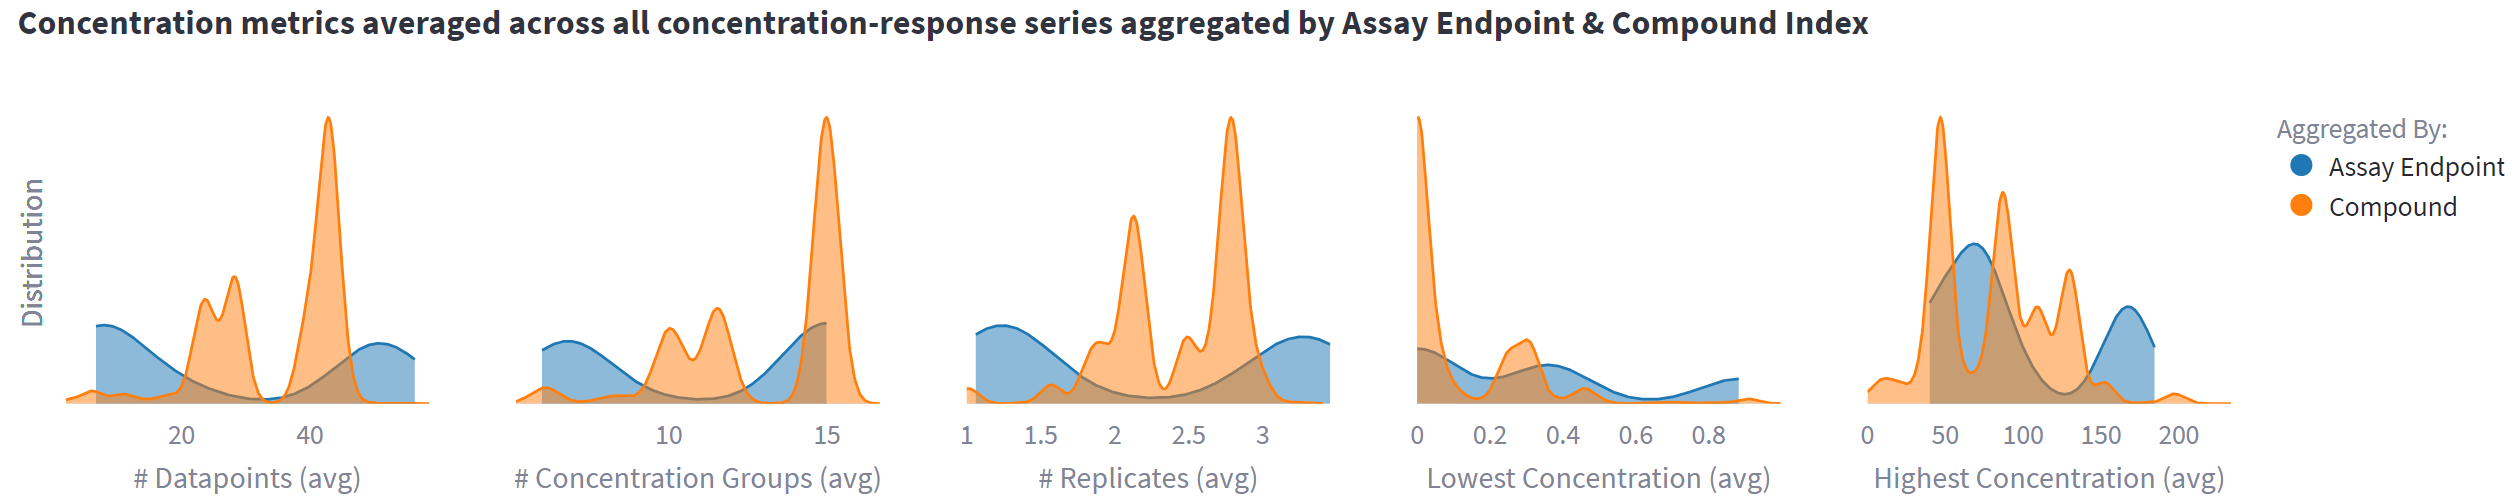
\includegraphics[width=1.0\textwidth]{figures/concentration_metric_distributions.png}  
    \caption{Concentration metrics averaged across all concentration-response series aggregated by assay endpoint (blue) and compound (orange). E.g., the first chart shows the distribution on the average number of datapoints across all assay enpoint $a_i \in A$ with $\frac{1}{|C_i|} \sum_{j} n_{\text{datapoints}_{i,j}}$ and across all compounds $c_j \in C$ with $\frac{1}{|A_j|} \sum_{i} n_{\text{datapoints}_{i,j}}$. Similarly, the process is repeated for the other metrics: $n_{\text{groups}_{i,j}}$, $n_{\text{replicates}_{i,j}}$, $min_{\text{conc}_{i,j}}$, and $max_{\text{conc}_{i,j}}$.
    }
~\label{fig:concentration_metric_distributions} 
\end{figure}


